% ОБЯЗАТЕЛЬНО ИМЕННО ТАКОЙ documentclass!
% (Основной кегль = 14pt, поэтому необходим extsizes)
% Формат, разумеется, А4
% article потому что стандарт не подразумевает разделов
% Глава = section, Параграф = subsection
% (понятия "глава" и "параграф" из стандарта)
\documentclass[a4paper,article,14pt]{extarticle}

\usepackage{etoolbox}
\cslet{blx@noerroretextools}\empty
\usepackage[backend=biber]{biblatex}
%\usepackage{autonum}

% Подключаем главный пакет со всем необходимым
\usepackage{spbudiploma}

% Пакеты по желанию (самые распространенные)
% Хитрые мат. символы
\usepackage{euscript}
% Таблицы
\usepackage{longtable}
\usepackage{makecell}
% Картинки (можно встявлять даже pdf)
\usepackage[pdftex]{graphicx}

\usepackage{amsthm,amssymb, amsmath}
\usepackage{textcomp}
\usepackage{amsmath}
\usepackage{comment}
\usepackage{svg}
%\usepackage{booktabs}



\addbibresource{bibliography.bib}

\begin{document}

% Титульник в файле titlepage.tex
% --------------------- Стандарт СПбГУ для ВКР --------------------------
% Автор: Тоскин Николай, itonik@me.com
% Если заметили ошибку, напишите на email
% Если хотите добавить изменение самостоятельно, GitHub: . PR-s welcome!
% Использованы материалы:
% habr.com/ru/post/144648/
% cpsconf.ru
% Текст:
% http://edu.spbu.ru/images/data/normativ_acts/local/20181030_10432_1.pdf
% Титульный лист:
% http://edu.spbu.ru/images/data/normativ_acts/local/20180703_6616_1.pdf
% -----------------------------------------------------------------------

% Титульный лист диплома СПбГУ
% Временное удаление foot на titlepage
\newgeometry{left=30mm, top=20mm, right=15mm, bottom=20mm, nohead, nofoot}
\begin{titlepage}
\begin{center}
% Первый символ съедается, первым знаком поставлен Ы
\textbf{Санкт--Петербургский}
\textbf{государственный университет}

\vspace{35mm}

\textbf{\textit{\large Ковалев Святослав Сергеевич}} \\[8mm]
% Название
\textbf{\large Выпускная квалификационная работа}\\[3mm]
\textbf{\textit{\large Прогнозирование временных рядов методами машинного обучения}}

\vspace{20mm}
% TODO: Узнать как правильно
Уровень образования: бакалавриат\\
Направление 01.03.02 «Прикладная математика и информатика»\\
«Прикладная математика, фундаментальная информатика и программирование»\\


% Научный руководитель, рецензент
% Сходить в уч отдел и узнать, правильно ли
\begin{flushright}
{Научный руководитель:} \\
% TODO: Узнать кафедру
профессор, кафедра компьютерных технологий \\ и систем, д.ф. - м.н.  Буре~Владимир Мансурович
\end{flushright}
\begin{flushright}
{Рецензент:} \\
% TODO: Узнать кафедру
профессор, кафедра компьютерных технологий \\и систем, д.ф. - м.н.  Буре~Владимир Мансурович
\end{flushright}

\vfill 

{Санкт-Петербург}
\par{2020 г.}
\end{center}
\end{titlepage}
% Возвращаем настройки geometry обратно (то, что объявлено в преамбуле)
\restoregeometry
% Добавляем 1 к счетчику страниц ПОСЛЕ titlepage, чтобы исключить 
% влияние titlepage environment
\addtocounter{page}{1}

% Содержание
\tableofcontents

\pagebreak
\specialsection{Введение}

Прогнозирование временных рядов играет важную роль в задачах экономики, финансов, прогнозировании погоды, анализе электроэнергии и прочих~\cite{ts25}.

Эта задача достаточно изучена для временных рядов, обладающих свойством стационарности - статистическим свойством, при котором основные характеристики ряда остаются неизменными со временем.
Стационарные ряды успешно прогнозируются линейными моделями, такими как ARIMA, GARCH, Exponential smoothing и другими.
Однако при работе с реальными данными временные ряды зачастую оказываются нестационарными.
Такие ряды стараются свести к стационарным и прогнозировать их уже известными методами.
В этой работе мы рассмотрим набор методов машинного обучения для прогнозирования временных рядов, не использующих свойство стационарности и применим описанные методы к данным цен биржевых торгов.
\par

Прогнозирование цен биржевых торгов позволяет крупным компаниям принимать стратегические решения, а частным трейдерам совершать выгодные сделки.
Цель этой работы - показать эффективность алгоритмов машинного обучения в вопросе прогнозирования цен биржевых торгов.
Чтобы показать эффективность алгоритмов, были использованы исторические данные, предоставляемые Yahoo Finance~\cite{yahoo},
по нескольким финансовым инструментам: цены на акции компании Tesla,
цена криптовалюты Bitcoin по отношению к доллару, цена доллара по отношению к евро и др.
\par

Помимо задачи прогнозирования временных рядов, также будет рассмотрен вопрос вопроизводимости вычислений.
Исследователи часто сталкиваются с двумя проблемами после завершения исследования.
\par
Во-первых, при разработке методов машинного обучения, исследователь получает положительные результаты в специально настроенном окружении.
Повторно настроить такое же окружение бывает просто невозможно и результат исследования невозможно переиспользовать для решения этой же задачи на продуктивном сервере.
\par
Во-вторых, зачастую обнаруживается, что метод, примененный для решения задачи, невозможно использовать для решения похожих задач.
Побочная цель этого исследования - обеспечить воспроизводимость представленного решения.
Для этого будут использоваться такой инструмент как Snakemake~\cite{snakemake}.

\pagebreak
\specialsection{Постановка задачи}

Даны временные ряды
\begin{equation}
    {X_{i} = \{x_{i,t}, t=\overline{1,k}\},\quad i=\overline{1,m}},
    \label{eq:equation}
\end{equation}
где $m$ - общее количество рядов, а размер всех рядов совпадает и равен $k$.
Цель - предсказать значение всех рядов с лагом $n$.

Для этого требуется построить такую модель $A(X_i)$, что
\begin{equation}
    A(X_i)=x_{i, k+n}.
    \label{eq:equation2}
\end{equation}

При этом модель должна при кросс-валидации минимизировать одну из метрик: MAE~\eqref{eq:mae}, MAPE~\eqref{eq:mape}, RMSE~\eqref{eq:rmse}.

MAE (Mean absolute error):
\begin{equation}
    MAE = \sum_{i=1}^{n} \frac{|y_i - x_i|}{n}
    \label{eq:mae}
\end{equation}

MAPE (Mean absolute percentage error):

\begin{equation}
    MAPE = \frac{1}{n} \sum_{i=1}^{n} \left| \frac{y_i - x_i}{y_i} \right|
    \label{eq:mape}
\end{equation}

RMSE (Root mean square error)
\begin{equation}
    RMSE = \sqrt{\sum_{i=1}^{n} \frac{(x_i - y_i) ^ 2}{n}}
    \label{eq:rmse}
\end{equation}

\pagebreak
\specialsection{Обзор литературы}

Научные работы о прогнозировании временных рядов появились еще в 1970 году в труде Бокса~\cite{box}.
Бокс рассматривает линейные стационарные модели и некоторые системы, сводящиеся к ним.
В частности, рассматривается модель ARIMA и ее производные, учитывающие сезонность и внешние факторы.
Немногим раньше появляется модель экспоненциального сглаживания~\cite{expsmooth}.
\par
Модели нейронных сетей появляются в 1987 году~\cite{firstnn} и сразу дают положительные результаты в области прогнозирования нелинейных систем.
Значительный вклад в развитие прогнозирования временных рядов внесла работа о LSTM~\cite{lstm} в 2012 году, в которой рассматривалась модификация рекурентной нейронной сети для задач распознавания речи.
Появляется множество статей, в которых модель LSTM с некоторыми модификациями превосходит в точности все ранее известные модели~\cite{lstm_ex1}~\cite{lstm_ex2}~\cite{lstm_ex3}.
\par
В это же время исследуется вопрос построения ансамблей моделей, когда на основе множества <<простых>> моделей обучается другой алгоритм регрессии, минимизирующий общую ошибку.
Такой подход применяли зарубежные исследователи в своей работе о построении ансамблевых моделей на основе глубоких нейронных сетей~\cite{ensemble_dl}.
Также бразильские исследователи сравнивали между собой ансамблевые модели, построенные на основе бэггинга, бустинга и стекинга для данных из области агрокультуры~\cite{ensemble_agri}.
\par
Помимо моделей прогнозирования большую роль в качество прогноза вкладывает предобработка данных и feature extraction. % TODO: написать про это


\pagebreak
\section{Прогнозирование временных рядов}

\subsection{Методы прогнозирования}

Для того, чтобы оценить качество моделей машинного обучения, необходимо построить множество моделей и сравнить их между собой для каждого конкретного ряда.
Для прогнозирования использовались как классические модели, такие как ARIMA, VAR, так и регрессионные модели машинного обучения - Wavelet и Stacking.
% Также были использованы различные нейронные сети для построения прогноза.
% При прогнозировании нейронными сетями использовались различные архитектуры с использованием как классических линейных слоев, так и рекуррентных ячеек LSTM и сверточных слоев.
Каждая из моделей сравнивалась с <<наивной>> моделью, которая предсказывала последнее известное значение на весь горизонт прогнозирования.

Ниже приводится краткий обзор каждого использованного метода.

\subsubsection{ARMA}
Рассмотрим модель ARMA:
\begin{equation}
    \label{eq:arma}
    X_{t}=c+\varepsilon _{t}+\sum _{i=1}^{p}\alpha _{i}X_{t-i}+\sum _{i=1}^{q}\beta _{i}\varepsilon _{t-i}
\end{equation}
где $c$ - константа, ${\varepsilon _t}$ - белый шум, а $\alpha_1, \dots, \alpha_p$ и $\beta_1, \dots, \beta_q$ - авторегрессионные коэффициенты и коэффициенты скользящего среднего.
\par
Такая модель может быть использована только для прогнозирования стационарных временных рядов.
Если же в задаче фигурирует нестационарный ряд, то используют модель ARIMA\@.

\subsubsection{ARIMA}
Модель ARIMA~\cite{arima} является классическим методом эконометрики для прогнозирования временных рядов.
Применение ARIMA для прогнозирования биржевых цен уже рассматривалось ранее~\cite{my_arima_article}.
\par
Модель ARIMA является производной от модели ARMA\@.
Для сведения нестационарного ряда к стационарному используется операция взятия разности или дифференцирование временного ряда.
Количество раз, которое исходный ряд дифференцируется перед тем как попасть в модель ARMA, является параметром, который обычно обозначают как $d$.

\subsubsection{VAR}
Модель VAR~\cite{var} позволяет находить линейные зависимости между компонентами многомерных временных рядов.
VAR - обобщение модели AR на многомерный случай.
Считается, что все рассматриваемые ряды зависимы, и что каждый из этих рядов нужно предсказать на $n$ шагов вперед.
Модель VAR можно записать следующим образом:
\begin{equation}
    y_{t}^{i}=a_{0}^{i}+\sum _{{j=1}}^{{k}}a_{{1j}}^{i}y_{{t-1}}^{j}+\sum _{{j=1}}^{{k}}a_{{2j}}^{i}y_{{t-2}}^{j}+\ldots +\sum _{{j=1}}^{{k}}a_{{pj}}^{i}y_{{t-p}}^{j}+\varepsilon _{{t}}^{i},
\end{equation}
где $y^{i}, i=1, \dots, k-i$-й временной ряд, а $a_{i}^{j}$ - коэффициенты авторегрессии.
Более компактно можно записать это уравнение в векторной форме:
\begin{equation}
    y_{t}=a_{0}+\sum _{{m=1}}^{p}A_{m}y_{{t-m}}+\varepsilon _{t},
\end{equation}
где $A_m$ - матрицы элементов $a^{i}_{mj}$
\par

\subsubsection{Wavelet}
В основе модели Wavelet~\cite{wavelet} лежит дискретное вейвлет преобразование.
Исходный ряд раскладывается на $k$ рядов, каждый из которых предсказывается по отдельности при помощи любой регрессионной модели (в нашем случае использовалась ARIMA), после чего выполняется обратное преобразование.
Использовалась реализация вейвлет функций из пакета PyWavelets~\cite{pywt}.
В качестве вейвлет-функций используются койфлеты, так как показали наилучший результат в результате полного поиска по сетке среди всех семейств вейвлетов, представленных в библиотеке.
Схему разложения можно видеть на рис.~\ref{fig:wavelet}.

\begin{figure}
    \begin{center}
        \scalebox{0.6} {
            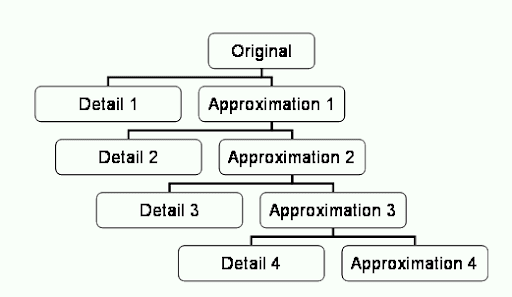
\includegraphics{images/wavelet}
        }
        \caption{
            Схема разложения исходного ряда. Ряды коэффициентов Approximation 4, Detail 1 - Detail 4 предсказываются регрессионной моделью.
            \label{fig:wavelet}
        }
    \end{center}
\end{figure}

\subsubsection{Naive one step}
Naive one step - <<наивная>> модель, которая предсказывает последнее известное значение на весь горизонт прогнозирования.
Такая модель не несет в себе никакой прогностической фунции, но с помощью нее можно определить, насколько хорошо построенная модель обобщает данные.
Так, если наивная модель показывает результаты какой-либо метрики лучше другой модели, это означает, что вторая модель недостаточно хорошо описывает данные в смысле выбранной метрики.

\subsubsection{Naive multi step}
Naive multi step - <<наивная>> модель, которая в качестве предсказания берет последние $n$ значений временного ряда.
Модель аналогична предыдущей модели, но лучше подходит под случай, когда в данных присутствует периодичность или сезонность.

\subsubsection{Stacking}
Stacking - ансамблевая модель, основанная на градиентном бустинге над решениями, описанными выше.
Как было показано, использование ансамблей решений помогают построить лучшее решение.
\par
В нашем случае в качестве модели, обобщающей предсказания, использовалась RandomForest из библиотеки scikit-learn, так как она дала лучшее качество, по сравнению с линейной регрессий (линейной комбинацией решений) и градиентным бустингом из библиотеки scikit-learn.
Для каждой модели производился полный перебор гиперпараметров по сетке.

\subsection{Оценка качества моделей}

Оценка качества моделей прогнозирования временных рядов отличается от оценки качества моделей регрессии в случаях, когда необходимо давать предсказание больше, чем на один шаг вперед.
\par
Пусть на вход модели поступает последние $k$ наблюдений ряда, а на выходе она предсказывает следующие $n$ значений.
При этом, чтобы избежать переобучения и не <<заглядывать в будущее>>, модель обучается только на данных, предшествующих последнему наблюдению, которое было передано в модель.
Тогда для каждого момента времени $t, t > k$ мы можем дать предсказание и сравнить его с фактическим значением ряда в этот же момент времени, например, посчитав среднеквадратичное отклонение или любую другую метрику, которая бы описывала качество предсказания.
Такой подход называется кросс-валидацией для временных рядов.
\par
Этот подход можно обобщить на случай, когда необходимо давать прогноз на каждый из $n$ шагов вперед.

Пусть, $X = \{x_i | i= \overline{1,m} \}$ - исходный временной ряд длины $m$.
Обозначим срез временного ряда от $i$ до $j$ как $X^j_i = \{x_t | t= \overline{i,j} \}, i < j$.

Тогда формально процесс кросс-валидации можно описать так:

\begin{enumerate}
    \item Выборка делится на тренировочную $X^j_i$ и тестовую $X^m_{j + 1}$.
    \item Модель обучается на тренировочной выборке.
    \item Тренировочная выборка прогнозируется на $n$ точек вперед.
    Обозначим предсказание $p_j^1$, если оно строится от точки $j$, как в~\eqref{eq:prediction} на $n$ шагов вперед.
    \begin{equation}
        \label{eq:prediction}
        p_j^1 = A(X^j_i)
    \end{equation}
    \item Считается целевая метрика~\eqref{eq:metric_calc}, сравнивая полученное предсказание с фактическими значениями в этот же момент времени.
    \begin{equation}
        \label{eq:metric_calc}
        M_j^1 = metric(p_j^1, X^{j+n}_j)
    \end{equation}
    \item Первая точка из тестовой выборки перемещается в тренировочную:
    \begin{equation}
        \label{eq:next_iter}
        \begin{aligned}
            i := i + 1, \\
            j := j + 1.
        \end{aligned}
    \end{equation} % может есть символ присвоения
    \item Повторяем процесс до тех пор, пока $j + n < m$, то есть пока в тестовой выборке больше, чем $n$ точек.
    \item Усредним значение полученного массива метрик.
\end{enumerate}

\begin{figure}
    \begin{center}
        \label{fig:cross-validation}
        \scalebox{0.6}{
            \includegraphics{images/cross-validation}
        }
        \caption{Иллюстрация кросс-валидации для временных рядов.}
    \end{center}
\end{figure}

\par
В предложенном алгоритме особое внимание стоит уделить процессу подсчета метрики.
Можно считать близость двух векторов (вектор предсказаний и вектор фактических цен), либо можно считать близость предсказания в последней точке прогноза.
\par
В первом случае мы оценим модель на то, насколько точно она прогнозирует общую картину изменения величины (скачки цен внутри периода, если говорить о биржевых цена).
\par
При этом, если задача состоит в предсказании $n$ значения, стоит считать метрику именно по последней точке предсказания.
В таком случае мы оценим насколько точно модель прогнозирует цену на заданный горизонт, игнорируя общую картину.

\par
В этой работе будем использовать второй подход, так как его проще визуализировать и интерпретировать.
То есть, оцениваться будет только прогноз модели в последний день прогноза.

В качестве метрики будем использовать:
\begin{itemize}
    \item Mean Absolute Error (MAE)~\eqref{eq:mae};
    \item Mean Absolute Percentage Error (MAPE)~\eqref{eq:mape};
    \item Root Mean Squared Error (RMSE)~\eqref{eq:rmse}.
\end{itemize}

\subsection{Воспроизводимость вычислений}

\subsubsection{Snakemake}
Для того, чтобы полученные результаты были достоверными и воспроизводимыми, а также чтобы полученные модели можно было использовать как фреймворк для произвольных данных в будущем, был построен конвейер (workflow) для обработки данных.
Для реализации конвейера использовался инструмент Snakemake~\cite{snakemake}.
Помимо Snakemake существует множество других инструментов, например Luigi~\cite{luigi}, Airflow~\cite{airflow} и многие другие.
Выбор пал на Snakemake, так как он очень прост в изучении, расширяет язык Python, но не связан с ним напрямую, и позволяет строить гибкие конвейеры, используя высокий уровень абстракции.
\par

Snakemake по своей сути очень похож на CMake, но более прост в использовании и адаптирован под создание конвейеров для анализа данных.
Большое внимание уделено вопросам масштабирования и параллельного исполнения, так как фрейворк часто используется для исследования задач биоинформатики, в которых зачастую фигурируют большие данные.
Как известно, в Python нет возможности эффективно производить параллельные вычисления средствами самого языка из-за GIL (Global Interpreter Lock).
Обычно эта проблема решается использованием отдельных процессов (workers), каждый из которых решает свою задачу, и которые способны общаться между собой через асинхронное хранилище (например, Redis).
Snakemake решает проблему масштабирования на своей стороне и предоставляет простой интерфейс для реализации параллельных вычислений как в рамках одной машины, так и для вычислительных кластеров.
\par

Snakemake позволяет определять <<правила>> (rules) для обработки данных.
Каждое правило может иметь входные и выходные файлы.
Правило должно генерировать из входного файла выходной.
Если snakemake не может найти входной файл в файловой системе, то ищется другое правило, которое генерирует этот файл.
Таким образом, получается ациклический граф работ (DAG), при помощи которого snakemake планирует и исполняет все необходимые работы для того, чтобы получить результат.
\par

Для конвейера можно определить параметры в специальном конфигурационном файле.
Например, это может быть URL-адрес с которого будут загружаться данные, параметры моделей, перечисление названий моделей, метрики для оценки качества моделей и прочее.
Параметризация конвейера позволяет быстро и качественно проводить исследование, не нарушая логику других экспериментов.
\par

Каждое правило в конвейере - python-скрипт, которому через аргументы командной строки передают пути к файлам и прочие параметры.
\par

Для решения задачи использовался граф работ, изображенный на рис.~\ref{graph_dag}.
\begin{figure}[ht]
    \begin{center}
        \scalebox{0.25}{
           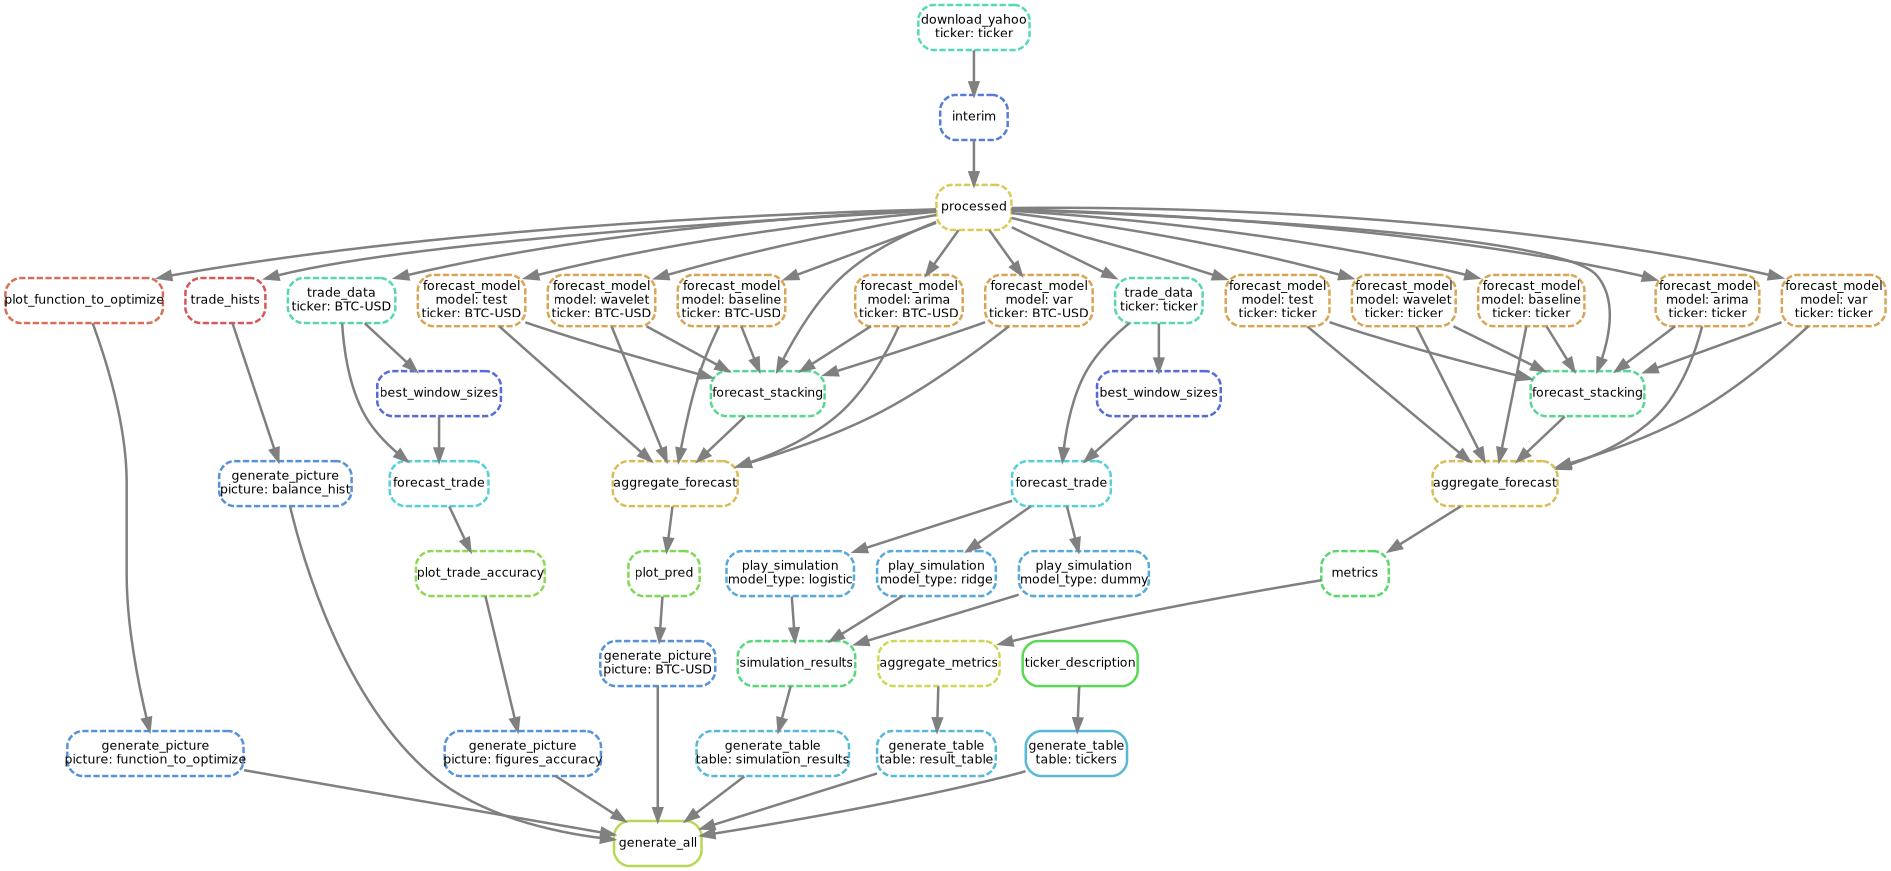
\includegraphics{images/dag}
        }
        \caption{
            \label{graph_dag}
                 Ациклический граф работ.
        }
    \end {center}
\end {figure}

\par
Весь исходный код можно использовать как внешнюю python-библиотеку, поверх которой возможно создать API и использовать как микросервис для предсказаний.

\subsubsection{Описание конвейера}
Можно выделить следующие шаги, исполняемые конвейером:

\begin{enumerate}
    \itemЗагружаются данные через API Yahoo finance по интересующим тикерам (котировкам) за указанный временной интервал.
    Для работы с API Yahoo finance используется python-библиотека yfinance.

    \item Преобразование исходных данных в удобный формат.
Обработку исходных данных можно поделить на следующие шаги:

    \begin{enumerate}
        \item raw - <<сырые>> данные, только что загруженные из источника.
        \item interim - данные, которые прошли первичную обработку.
    В данных отсутствуют лишние колонки и строки.
    Набор исходных файлов агрегируется в один, или наоборот, исходный файл разбивается на несколько логических файлов.
        \item processed - готовый датасет, который готов к загрузке в модель.
    Такие данные получаются из interim данных, в которых заполняются пропуски и генерируются дополнительные признаки.
    \end{enumerate}
    Использование таких шагов для обработки позволяет реже перезапускать весь конвейер и упрощает обработку данных.
    \item Использование моделей для построения прогнозов по заданным датам и генерации тестовой выборки.
Модели дают предсказание от стартовой даты до конечной даты, которые указываются в конфигурационном файле.
Также для моделей указывается горизонт прогнозирования.
Итоговое предсказание модели представляет из себя таблицу, у которой в строках указаны даты, от которых ведется предсказание, а порядковый номер столбца означает горизонт прогнозирования.
Например, если предсказание необходимо дать с 1 января 2019 года по 30 января 2020 года с горизонтом в 3 дня, то в таблице будет 30 строк и 3 столбца.
Тестовые значения генерируются аналогичным образом, только вместо прогноза используются настоящие значения временных рядов.
    \item Полученные данные используются для генерации графиков и подсчета метрик.
На этом этапе читаются все предсказания, полученные на прошлом этапе и идет оценка результатов прогнозирования.
По результатам проверки сохраняется таблица со всеми полученными метриками.
Также отрисовываются графики по каждому прогнозу~\ref{fig:btc-usd}.
    \item Генерируется код LaTeX для вставки графиков и таблиц с результатами.
На этом шаге используются графики и таблицы с прошлого шага.
Таблицы из формата csv транслируются в LaTeX\@.
Пути до изображений также вставляются в LaTeX\@.
Параметры таблиц и изображений (например, ширина столбцов, расположение на странице, label) лежат в отдельном конфигурационном файле.
    \item LaTeX шаблон компилируется и генерирует pdf-файл с оформленными графиками и таблицами.
В случае проведения нового эксперимента, добавления новой модели или использования новых данных, запуском одной команды pdf-файл собирается заново, из-за чего ошибки в цифрах в итоговом документе исключены.
\end{enumerate}
\par

Также используется примитивное версионирование: результаты каждого запуска сохраняются в отдельную папку и архивируются, сохраняя временную метку и автора запуска конвейера.
\par
В случае работы нескольких человек над проектом возможна организация версионирования через облачное хранилище.
После каждого запуска идет загрузка полученного архива в облачное хранилище, а на локальную машину загружаются все отсутствующие исследования, которые были проведены до этого момента.
Такой подход решает проблему совместной работы над проектом и позволяет не потерять полученные результаты.

\pagebreak
\section{Эксперимент}

\subsection{Описание исходных данных}
Были взяты данные о ценах и объемах биржевых торгов с Yahoo Finance~\cite{yahoo}.
Yahoo Finance предоставляет данные о <<тикерах>> (ticker) - торговых парах.
Каждый тикер имеет свой код. 
Например, акции компании Tesla, торгующиеся в долларах, имеют код TSLA\@.
Тикеры, которые были взяты для анализа, представлены в таблице~\ref{tab:ticker_table}.
\input{../reports/latex/tables/tickers.tex}

\par
API Yahoo Finance предоставляет по умолчанию данные за последние три года с частотой в один день. 
За каждый день предоставляются данные о минимальной и максимальной цене сделки, об открывающей и закрывающей цене торгов, а также об объеме торгов.
Будем использовать эти данные для обучения.
\par
Для предсказания был выбран промежуток c 1 февраля 2021 года по 30 марта 2021 года.
Прогноз строился на 10 дней вперед.

\subsection{Подготовка данных}

\subsubsection{Этап предобработки raw}
Этот этап необходим для того, чтобы сохранить загруженные данные.
В случае, если дальше в конвейере произойдет ошибка, можно будет использовать уже загруженные данные.

\subsubsection{Этап предобработки interim}
На этом этапе выбирается нужный временной промежуток в данных.
Например, если были загружены данные за последние 10 лет, а для прогнозирования необходимо использовать данные за последний год, то это отсечение ненужных данных произойдет на этом этапе.
\par

Если в данных есть пропуски, то они заполняются последним известным значением.
Если пропущены первые значения в ряде, они заполняются первым известным значением.

\subsubsection{Этап предобработки processed}

На этом этапе из данных выделяются необходимые столбцы, а именно:
\begin{enumerate}
    \item Open - цена первой сделки за выбранный промежуток торгов.
    \item Close - цены последней сделки за выбранный промежуток торгов.
    \item High - наивысшая цена за выбранный промежуток торгов.
    \item Low - наименьшая цена за выбранный промежуток торгов.
\end{enumerate}
\par

Это необходимо сделать, так как в исходных данных есть лишние столбцы, в которых нет нужды.

\subsection{Результаты}
Для каждого временного ряда применялась каждая из моделей.
Модель VAR применялась сразу для всех временных рядов.
Сравнение результатов происходило по метрикам MAE~\eqref{eq:mae}, MAPE~\eqref{eq:mape} и RMSE~\eqref{eq:rmse}.

Результаты можно наблюдать в таблице~\ref{tab:results_table}.
Также результат прогноза для тикера BTC-USD можно видеть на рис.~\ref{fig:btc-usd}.
\pagebreak
\input{../reports/latex/tables/result_table.tex}
\input{../reports/latex/pictures/BTC-USD.tex}

Как видно из таблицы и графика, наивная модель дает результат, который не всегда получается превзойти.
Это объясняется тем, что на ряд влияют внешние неизвестные факторы, которыми нельзя пренебречь.

\subsection{Моделирование торговли на бирже}
\subsubsection{Постановка задачи}

Помимо классической задачи прогонозирования временных рядов может быть полезно использовать альтернативный подход.
Будем моделировать торговлю на бирже.
Пусть в нулевой момент имеется $C$ долларов, на которые можно купить актив по цене $price_i$ в момент времени $i$.
Торговля продолжается на протяжении определенного периода (неделя, месяц, год), в конце которого все активы продаются по текущей цене.
Задача - максимизировать итоговое количество долларов.
Также для удобства будем пользоваться формулой~\eqref{eq:profit}

\begin{equation}
    profit = \frac{revenue - cost}{cost} * 100
    \label{eq:profit}
\end{equation}

Сведем задачу к задаче классификации.
Каждую точку исходного временного ряд разметим на три класса: «sell», «buy», «hold»:

\begin{itemize}
    \item sell - означает, что скоро цена значительно снизится, а следовательно нужно продавать активы;
    \item buy - означает, что скоро цена значительно повысится, а следовательно нужно покупать активы;
    \item hold - означает, что цена в ближайшее время значительно не изменится, а значит ничего делать не нужно.
\end{itemize}

Выберем горизонт прогнозирования $n$ и сформируем обучающую выборку.
Для каждой точки посчитаем изменение цены в процентах в момент $i$~\eqref{eq:delta}

\begin{equation}
    \Delta p_i = \frac{price_{i + n} - price_{i}}{price_{i}} * 100
    \label{eq:delta}
\end{equation}

Выберем порог $t$, начиная с которого будем считать, что изменение цены значительное и выберем класс для каждой точки по правилу~\eqref{eq:equation3}

\begin{equation}
class_i =
 \begin{cases}
     sell &\text{if $ \Delta  p_i < -t$}
     \\
     buy &\text{if $\Delta p_i > t$}
     \\
     hold &\text{if $|\Delta p_i| < t$}
 \end{cases}
\label{eq:equation3}
\end{equation}

Порог $t$ можно выбирать вручную в зависимости от целей трейдера, но на случай, когда необходимо проанализировать большое количество временных рядов, хотелось бы иметь алгоритм автоматического подбора порога $t$.
\par
Для того, чтобы в дальнейшем было проще оценивать результаты задачи классификации, будем исходить из предпосылки, что данные разбиты на равные классы.

Будем решать задачу одномерной оптимизации, в которой $t$ выступает в качестве независимой переменной.

Введем понятие сбалансированности.
Пусть есть выборка из $N$ элементов, каждый из который принадлежит одному из $k \in K$ классов.
Для каждого класса можно посчитать его долю от общего числа элементов:

\begin{equation}
    \{ \frac{n_1}{N}, \frac{n_2}{N}, \dots , \frac{n_K}{N} \}
    \label{eq:fractions}
\end{equation}

Будем называть классы сбалансированными, когда

\begin{equation}
    \frac{n_1}{N} \approx \frac{n_2}{N} \approx \dots \approx \frac{n_K}{N}
    \label{eq:balanced}
\end{equation}

В нашем случае имеем 3 класса, соответственно стремимся к тому, чтобы доля каждого класса составляла $\frac{1}{3}$ от общего числа примеров.

Введем функционал качества:

\begin{equation}
    J=\sum{(\frac{n_i}{N} - \frac{1}{K}) ^ 2}
    \label{eq:error_func}
\end{equation}

где $n_i$ - количество элементов, принадлежащих классу $i, i < K$.
Будем считать, что разбиение на классы зависит от порога $t$.
Тогда можем автоматически выбирать $t$ как решение задачи оптимизации:

\begin{equation}
    t_{opt} = argmin_t J
    \label{eq:equation4}
\end{equation}

Полученная оптимизационная задача решается методом нулевого порядка (например, методом золотого сечения).

Однако для целевой функции не была доказана выпуклость, поэтому могут возникнуть случаи, когда в результате оптимизации будет достигнут локальный минимум.
Пример целевой функции приведен на рис.~\ref{fig:function_to_optimize}

\input{../reports/latex/pictures/function_to_optimize.tex}

Обычно локальный минимум достигается, когда вся обучающая выборка состоит из одного и того же класса, а параметр $t$ либо отрицателен, либо очень большой.
Чтобы избежать таких случаев рекомендуется ставить ограничения на оптимизационную задачу.
Из постановки задачи следует, что параметр $t$ лежит в промежутке $(0, 100)$.
Однако чаще всего разумные значения параметра лежат в промежутке $(0, 50)$.
Наложим эти ограничения на оптимизационную задачу, а также будем оценивать, какое количество классов выделил алгоритм.
Если не был выделен какой-то класс, то будем сужать промежуток вдвое (уменьшая верхнюю границу).

\par
Полученный метод был применем ко всем выбранным временным рядам.
Пример приведен на рис.~\ref{fig:balance_hist}

\input{../reports/latex/pictures/balance_hist.tex}

Таким образом, мы получили размеченную выборку и теперь можем решать задачу классификации.

\subsubsection{Построение моделей классификации}

Поставим задачу обучения с учителем для полученного датасета.
Необходимо построить функцию $f(x)=d, d \in \{sell, buy, hold\}$, которая на вход получает информацию о временом ряде, а на выходе принимает решение о продаже, покупке или удержании активов.

Задачу классификации можно решать множеством методов.
При проведении эксперимента использовались модели линейной регрессии, случайного леса и логистической регрессии.

Остается открытым вопрос о том, какую информацию об исходном ряде передавать в модель.
Обычно берут окно фиксированной длины $w$ и в качестве входных данных передают последние $w$ значений временного ряда.
Длина окна - гиперпараметр модели, который необходимо подобрать.

При подборе гиперпараметра будем исходить из горизонта прогнозирования $n$.
Будем оценивать качество модели для каждого значения $w$~\eqref{eq:equation5}

\begin{equation}
    \label{eq:equation5}
    w \in \left[ n - \frac{n}{2}; n + \frac{n}{2} \right].
\end{equation}

Оценивать качество моделей будем при помощи метрики accuracy, используя кросс-валидацию для временных рядов, как это было описано ранее.

Сравнивать качество метрики можно со случайным угадыванием, то есть считаем, что какая-то модель в каждой точке кросс-валидации дала точность $\frac{1}{3}$.

Результаты для одного из рядов можно увидеть на рис.~\ref{fig:figures_accuracy}
\input{../reports/latex/pictures/figures_accuracy.tex}

\subsubsection{Симуляция биржевых торгов}

Будем считать, что у трейдера есть возможность купить или продать активы в конце торгового дня (ориентируемся на показатель Close).

Модель предсказывает одно из трех значений: sell, buy, hold.
Трейдер действует точно по инструкции:

\begin{itemize}
    \item sell - продать все имеющиеся активы, если они есть;
    \item buy - купить активы на все деньги;
    \item hold - ничего не делать.
\end{itemize}

Будем считать, что на бирже всегда есть необходимый объем активов и что цена не меняется в зависимости от приобретенных активов.
\par

Так продолжается на протяжении какого-то периода (неделя, месяц или год), а в конце продаются все активы, вне зависимости от цены, и подсчитывается итоговая стоимость портфеля.
Чем дольше выбирается период, тем более точно можно оценить качество алгоритма.
\par

Помимо трейдеров, которые торгуют согласно прогнозам алгоритмов, введем еще двух трейдеров, чтобы оценить качество алгоритмов.
Введем трейдера, которому достоверно известна информация о будущем (идеальная модель).
Также введем трейдера, который случайно принимает решение.
Для того, чтобы уменьшить влияние случайности, посчитаем результаты для ста таких трейдеров и усредним их результат ($profit$).

Результаты представлены в таблице~\ref{tab:simulation_results_table}.
\input{../reports/latex/tables/simulation_results.tex}

\pagebreak

\section{Прогнозирование цен биржевых торгов на бирже СПбМТСБ}

Санкт-Петербургская Международная Товарно-Сырьевая Биржа \linebreak
(СПбМТСБ)~\cite{spimex} является основной площадкой для торгов нефтепродуктами в России, на которой происходит подавляющее число операций по их покупке и продаже.
Так, по итогам 2018 года, каждая четвертая тонна бензина, реализованная в РФ, торговалась на СПбМТСБ.
Помимо бензина разных марок, здесь также продаются дизельное топливо, керосин и мазут.
СПбМТСБ функционирует пять дней в неделю с понедельника по пятницу, с выходными в субботу и воскресенье, а также в государственные праздники.

Биржевая торговля осуществляется в режиме двойного встречного анонимного аукциона, при котором продавец и покупатель не видят друг друга и не могут сговориться о цене.
Сделка заключается автоматически при пересечении условий во встречных анонимных заявках.
Благодаря особой организации биржевых торгов, они позволяют определять справедливую рыночную стоимость товаров.

Компания ПАО <<Газпром нефть>> была заинтересована в том, чтобы прогнозировать цены реализации ряда нефтепродуктов на 14 дней вперед.

В качестве исходных данных были предоставлены данные о средневзвешенных ценах торгов по необходимым инструментам, а также некоторые внешние данные, в которых содержится информация об экономических процессах, влияющих на ценообразование.


Для решения задачи были использованы описанные выше алгоритмы.
В качестве метрики использовалась MAPE~\eqref{eq:mape}.

Результаты предоставлены в таблице~\ref{tab:exchange_results}.

\begin{center}
        \begin{longtable}{|p{3.5cm}|p{2cm}|p{2cm}|p{2cm}|p{2cm}|}
            \hline
        \textbf{} & \textbf{arima} & \textbf{wavelet} & \textbf{var} & \textbf{stacking} \\
        \hline
        АИ-92 ОНПЗ & 2.95 & 2.54 & 3.33 & 1.83 \\
        \hline
        АИ-92 МНПЗ & 3.61 & 3.11 & 2.93 & 1.85 \\
        \hline
        АИ-92 ЯНОС & 4.46 & 2.92 & 3.25 & 1.98 \\
        \hline
        АИ-95 ОНПЗ & 3.63 & 3.39 & 3.81 & 2.05 \\
        \hline
        АИ-95 МНПЗ & 4.91 & 3.66 & 3.54 & 2.11 \\
        \hline
        АИ-95 ЯНОС & 4.9 & 3.65 & 3.94 & 1.91 \\
        \hline
        ДТ ОНПЗ & 1.88 & 1.65 & 2.14 & 1.08 \\
        \hline
        ДТ МНПЗ & 5.71 & 1.74 & 2.07 & 1.13 \\
        \hline
        ДТ ЯНОС & 2.38 & 1.86 & 2.29 & 1.18 \\
        \hline
        Мазут ОНПЗ & 16.75 & 14.5 & 15.94 & 6.39 \\
        \hline
        Мазут МНПЗ & 13.3 & 12.58 & 12.97 & 5.58 \\
        \hline
        Мазут ЯНОС & 11.86 & 11.79 & 11.32 & 5.33 \\
        \hline
        ТС-1 ОНПЗ & 3.46 & 3.0 & 3.01 & 1.96 \\
        \hline
        ТС-1 ЯНОС & 2.29 & 2.16 & 2.88 & 1.14 \\
        \hline
    \end{longtable}
%    \caption{}
    \label{tab:exchange_results}
\end{center}

\pagebreak
\specialsection{Выводы}

Таким образом, использованные методы прогнозирования в некоторых случаях дают прогноз лучше, чем наивное или случайное предсказание.
Учитывая высокую волатильность рынков, этот результат является значимым.
Использованные подходы прогнозирования универсальны и их можно применять для предсказания любых других временных рядов, например, в задачах прогнозирования погоды, городских пробок и различных экономических показателей.
Полученные результаты можно улучшить, если учитывать внешние факторы, объясняющие исходный ряд.

\par
Подход, связанный с симуляцией биржевых торгов, также дает положительный результат для большинства рядов.

\par
В дальнейшем исследование может получить несколько векторов развития.
\par
Во-первых, могут быть рассмотрены другие прогнозные модели.
Например, можно использовать нейросетевые методы, или другие техники построения ансамблей.
\par
Во-вторых, можно глубже исследовать вопрос предобработки исходных данных.
Данные можно сглаживать при помощи скользящей средней, медианного фильтра или вейвлет-фильтра.
Также можно рассмотреть различные декомпозиции временных рядов, например CEEMDAN~\cite{lstm_ex2}.
\par
В-третьих, результаты можно значительно улучшить, если обогатить модели внешними данными, которые бы объясняли исходный ряд.
Например, акции Tesla связаны с высказываниями основателя компании в Twitter.
Можно провести сентимент-анализ сообщений в Twitter, и использовать полученные результаты как экзогенные признаки для модели Stacking.

\pagebreak

\printbibliography[heading=bibintoc]
% Библиография в cpsconf стиле
% Аргумент {1} ниже включает переопределенный стиль с выравниванием слева
\begin{comment}
    \begin{thebibliography}{1}
    \bibitem{ts25} J.G. De Gooijer, R.J. Hyndman, 25 years of time series forecasting, Int. J. Forecast. 22 (3) (2006) 443–473.
    \bibitem{box} G.E.P. Box, G. Jenkins, Time Series Analysis, Forecasting and Control, Holden-Day, San Francisco, CA (1970)
    \bibitem{expsmooth} Forecasting Sales by Exponentially Weighted Moving Averages, Peter R. Winters
    \bibitem{ar} Fitting autoregressive models for prediction, H Akaike - Annals of the institute of Statistical Mathematics, 1969 - Springer
    \bibitem{firstnn} Lapedes, A, and Farber, R. Nonlinear signal processing using neural networks: Prediction and system modelling. United States: N. p., 1987. Web.
    \bibitem{lstm} LSTM Neural Networks for Language Modeling, Martin Sundermeyer, Ralf Schlüter, Hermann Ney, 2012
    \bibitem{lstm_ex1} Applying LSTM to Time Series Predictable Through Time-Window Approaches, Felix A. GersDouglas EckJürgen Schmidhuber
    \bibitem{lstm_ex2} Financial time series forecasting model based on CEEMDAN and LSTM, Jian Cao, Zhi Li, Jian Li, 2018
    \bibitem{lstm_ex3} A Comparison of ARIMA and LSTM in Forecasting Time Series, Sima Siami-Namini, Neda Tavakoli, Akbar Siami Namin
    \bibitem{ensemble_dl} Ensemble deep learning for regression and time series forecasting, Xueheng Qiu; Le Zhang; Ye Ren; P. N. Suganthan; Gehan Amaratunga, 2014
    \bibitem{ensemble_agri} Ensemble approach based on bagging, boosting and stacking for short-term prediction in agribusiness time series, Matheus Henrique Dal Molin Ribeiro, Leandro dos Santos Coelho, 2020
    \bibitem{arima} Магнус Я. Р., Катышев П. К., Пересецкий А. А. Эконометрика. Начальный курс.. М.: Дело, 2004. 576 с.
    \bibitem{var} Носко В.П. Эконометрика. Введение в регрессионный анализ временных рядов
    \bibitem{snakemake} Köster, Johannes and Rahmann, Sven. “Snakemake - A scalable bioinformatics workflow engine”. Bioinformatics 2012.
    \bibitem{wavelet} Wang, F.; Yu, Y.; Zhang, Z.; Li, J.; Zhen, Z.; Li, K. Wavelet Decomposition and Convolutional LSTM Networks Based Improved Deep Learning Model for Solar Irradiance Forecasting. Appl. Sci. 2018, 8, 1286.
    \bibitem{yahoo} Yahoo Finance [Электронный ресурс] // Yahoo Finance. \url{URL:  https://finance.yahoo.com/} (дата обращения: 20.12.2020).
    \bibitem{my_arima_article} Ковалев С.С. Прогнозирование средневзвешенной цены торгов нефтепродуктами на бирже классическими методами анализа временных рядов. // Процессы управления и устойчивость. 2020. №51.
    \bibitem{pywt} Gregory R. Lee, Ralf Gommers, Filip Wasilewski, Kai Wohlfahrt, Aaron O’Leary (2019). PyWavelets: A Python package for wavelet analysis. Journal of Open Source Software, 4(36), 1237
    \bibitem{luigi} https://github.com/spotify/luigi
    \bibitem{airflow} https://airflow.apache.org/
    \end{thebibliography}
\end{comment}

\end{document}